\documentclass[10pt]{article}
\usepackage{tikz}
\usetikzlibrary{shapes}
\pagestyle{empty}

\begin{document}

\begin{center}
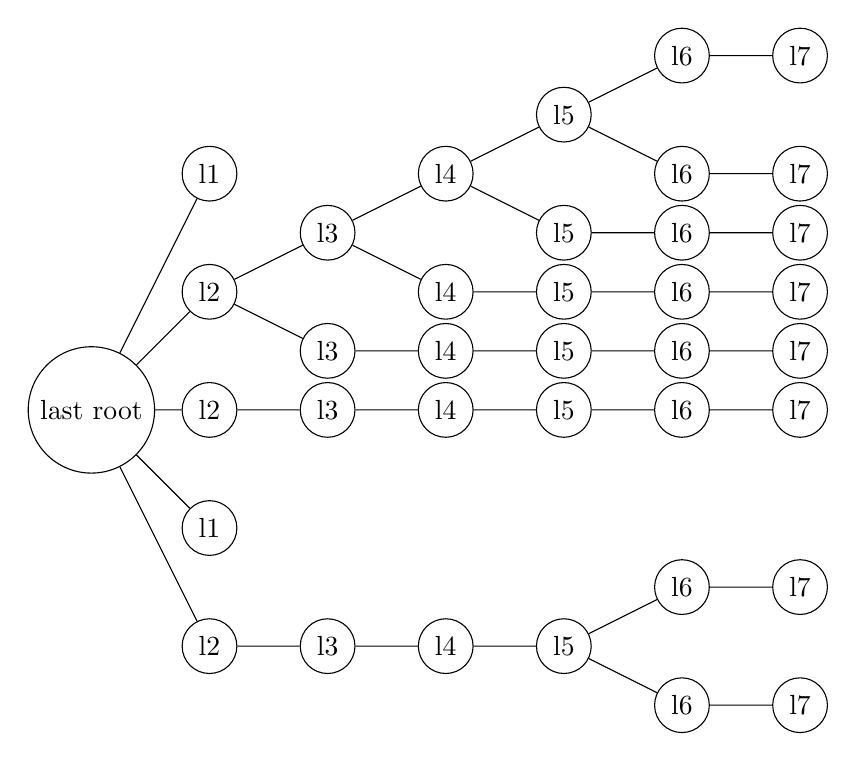
\begin{tikzpicture}
[grow'=right]
\tikzstyle{every node}=[circle,draw]
\node {last root}
    child {node {l1}}
    child {node {l2}
        child {node {l3}
            child {node {l4}
                child {node {l5}
                    child {node {l6}
                        child {node {l7}}
                    }
                    child {node {l6}
                        child {node {l7}}
                    }
                }
                child {node {l5}
                    child {node {l6}
                        child {node {l7}}
                    }
                }
            }
            child {node {l4}
                child {node {l5}
                    child {node {l6}
                        child {node {l7}}
                    }
                }
            }
        }
        child {node {l3}
            child {node {l4}
                child {node {l5}
                    child {node {l6}
                        child {node {l7}}
                    }
                }
            }
        }
    }
    child {node {l2}
        child {node {l3}
            child {node {l4}
                child {node {l5}
                    child {node {l6}
                        child {node {l7}}
                    }
                }
            }
        }
    }
    child {node {l1}}
    child {node {l2}
        child {node {l3}
            child {node {l4}
                child {node {l5}
                    child {node {l6}
                        child {node {l7}}
                    }
                    child {node {l6}
                        child {node {l7}}
                    }
                }
            }
        }
    };
\end{tikzpicture}
\end{center}

\end{document}
